\chapter[Methods]{Methods}
\section{Cyclus}
\subsection{Open Source}

\paragraph{The open source aspect of Cyclus allows for a breadth of scenarios}

\subsection{Modular}

\paragraph{Each facility and toolkit in Cyclus is made to be modular such that they can be employed as necessary}

\subsection{Archetypes}

\paragraph{Archetypes are a general form of facility so multiple forms of prototypes do not have to be developed.}

\section{Pyre}

\subsection{Structure of Pyre}
\paragraph{Governing Pyre Class}

\begin{figure}
	\centering
	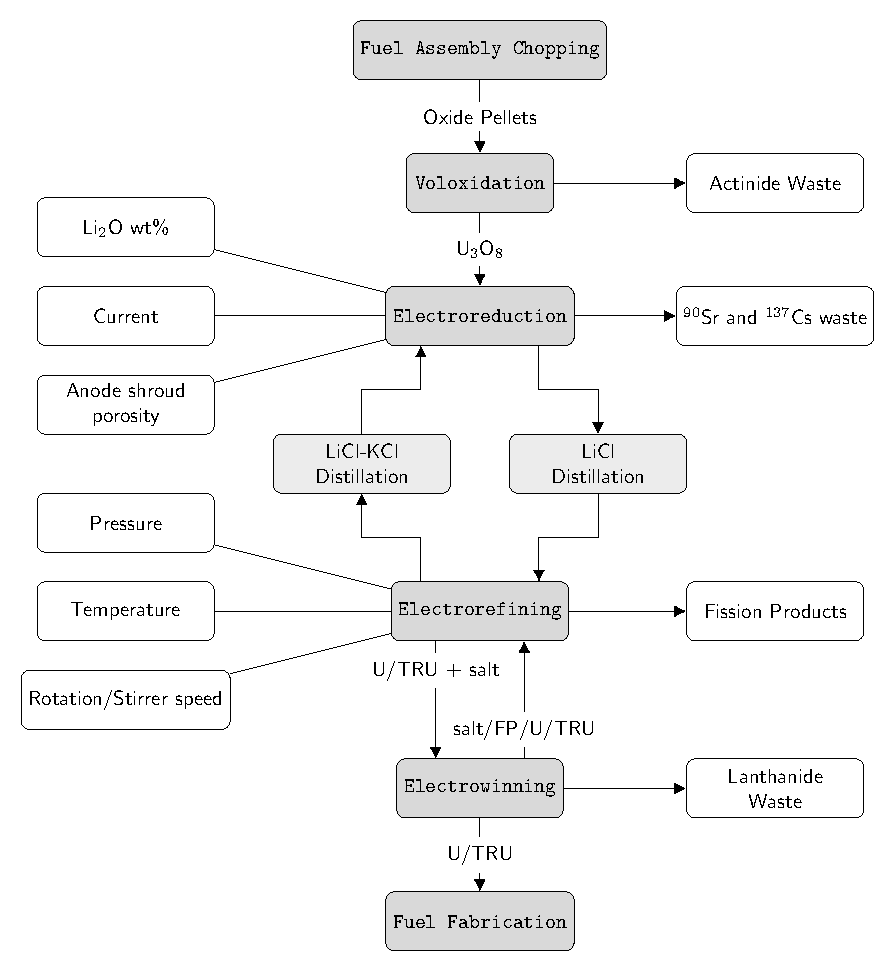
\includegraphics[width=0.95\linewidth]{images/flowchart}
	\caption{PyRe material flowchart \cite{borrelli_approaches_2017}.}
	\label{fig:flowchart}
\end{figure}

\paragraph{Diverter}

\paragraph{Cumulative Sum}

\paragraph{Material Trading}

\subsection{Material Balance}
\paragraph{Voloxidation}

\gls{LWR} fuel must be treated and separated before proceeding with electrolytic processes. Uranium dioxide heated to 
500$^{\circ}$C is converted to $U_3O_8$ while noble gases, carbon, and tritium are collected to decay in storage. 
Actinides are also converted to their stable oxide forms and a majority are removed \cite{flowsheet_1998,jubin_spent_2009}. 
Heating uranium dioxide above 800$^{\circ}$C increases voloxidation throughput.
Cycling oxidants between H$_2$ and air also improves the U$_3$O$_8$ reaction rate \cite{jubin_spent_2009}.

\begin{figure} 
	\centering
	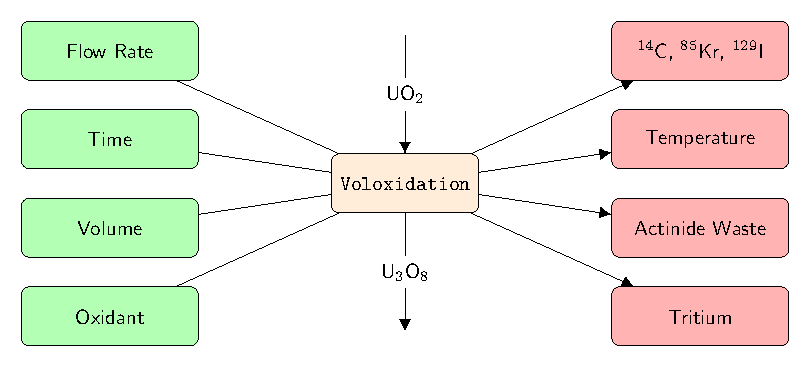
\includegraphics[width=0.9\linewidth]{images/volox}
	\caption{Voloxidation material balance area \cite{jubin_spent_2009}.}
	\label{fig:volox}
\end{figure}

\paragraph{Electroreduction}

The oxidant is converted into metallic fuel through electroreduction to be further refined through electrorefining and electrowinning. 
Yellowcake, created in voloxidation, enters the cathode, a negatively charged metal basket. 
A current density between 100 and 500 mA/cm$^2$ is applied to the anode in a molten LiCl salt. 
The electrolytic reduction process primarily results in diffusion of Cs, Ba and Sr, along with reduction and conversion of zirconium into metallic form \cite{choi_electrochemical_2015,flowsheet_1998}.
Electroreduction can further improve its throughput by adding Li$_2$O as a catalyst; this catalyst also prevents dissolution 
of the anode \cite{choi_electrochemical_2015}. Since Li$_2$O is used to speed up the reaction,
the operators could add more oxide than reported to \gls{IAEA}. More frequent shipments 
of lithium oxide can be tracked as an observable to match records.

\begin{figure} 
	\centering
	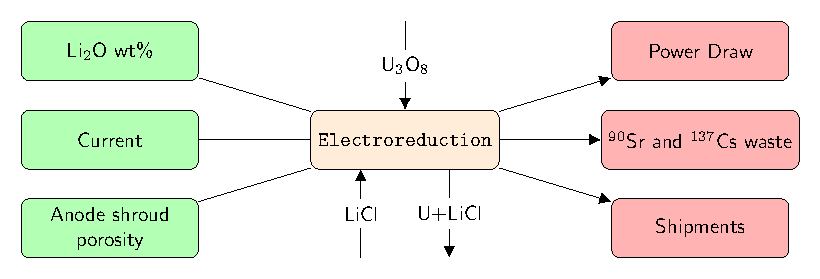
\includegraphics[width=0.9\linewidth]{images/reduction}
	\caption{Reduction material balance area \cite{lee_advanced_2008}.}
	\label{fig:reduction}
\end{figure}

\paragraph{Electrorefiner}

Once in metallic form, electrorefining electrochemically separates uranium and  for fuel fabrication.
The uranium and salt mixture from reduction is fed into an anode basket suspended in a graphite cathode. 
A LiCl-KCl eutectic is used as an electrolyte above 500$^{\circ}$C \cite{flowsheet_1998,lee_korean_2011}. 
Uranium dissolves at the anode to recombine at the cathode as metallic uranium.
\glsreset{TRU} 
Waste \glspl{TRU} and lanthanides are in a soluble chloride form  while fission products and cladding remain in the anode
basket. Finally, actinides and fission products are removed from the cladding electrochemically \cite{lee_korean_2011}.

Lee et al. \cite{lee_advanced_2008} show decreasing system pressure improves removal efficiency. 
Temperature, however, exhibits the opposite effect: as temperature decreases so does salt removal. This comes into effect 
particularly depending on material choice of instrumentation and containment \cite{lee_advanced_2008}. 
Iron, for example, limits operating temperature because a eutectic forms at 725$^{\circ}$C \cite{chapman_revision_1984}.
In facilities where iron equipment is present, temperatures are limited to 700$^{\circ}$C, hindering efficiency. 
Cathode arrangement and anode rotation speed also affect the collection of uranium 
dendrites \cite{lee_advanced_2008}. A central stirrer mixes uranium dendrites stuck on 
the vessel, improving separation efficiency and increasing throughput. 

\begin{figure}
	\centering
	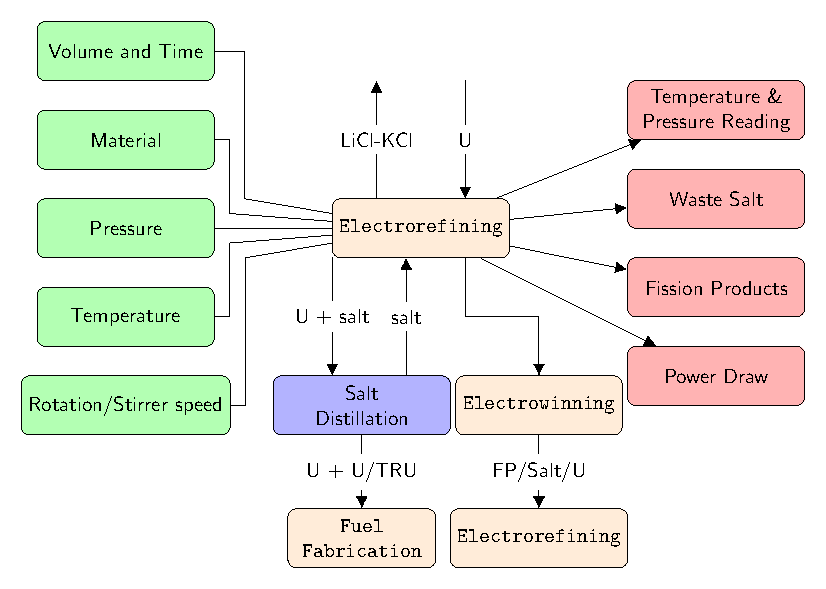
\includegraphics[width=0.85\linewidth]{images/refining}
	\caption{Refining material balance area \cite{lee_advanced_2008}.}
	\label{fig:refining}
\end{figure}

The electrorefining process also produces a fission product waste stream which requires monitoring. 
The following products are produced and tracked in \gls{PyRe} at this step: Tc, Ag, Pd, Rh, Ru, Mo and Zr \cite{flowsheet_1998}. 
Uranium and \gls{TRU} product streams separated at this stage are sent to fuel fabrication, while the remaining salt is reformed as an oxidant and recirculated.
Separation efficiencies are taken after recirculation, and treated as a once-through cycle. Cyclus' time step
is not detailed enough to benefit from analyzing intra-batch processes. Therefore, only end-state efficiencies are used rather than an explicit model.

\paragraph{Electrowinner}

Molten salt containing \glspl{TRU} from electrorefining is separated through electrowinning. This process separates trace uranium quantities, lanthanides and fission products. 
At 500$^{\circ}$C there is approximately 99 wt\% reduction in actinides and lanthanides \cite{flowsheet_1998}. 
Throughput also depends on material choice for the inert electrodes, impacting separation 
efficiency \cite{koyama_development_2012}. A shroud surrounds the anode to provide a path for O$^{2-}$ ions to the anode and 
prevent Cl$_2$ from corroding the anode \cite{kim_development_2013,choi_electrochemical_2015}. Optimum operating current 
depends on material choice for the anode shroud since a nonporous shroud limits ion pathways to the anode contact points.
Higher porosity corresponds to free ion paths and a higher current. Increased currents reduce the separation time for electroreduction and electrowinning \cite{choi_electrochemical_2015}.

\begin{figure} 
	\centering
	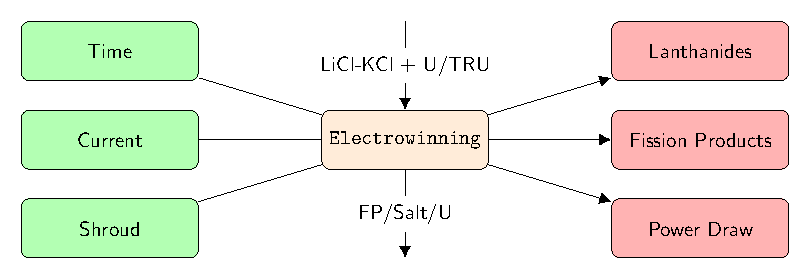
\includegraphics[width=0.8\linewidth]{images/winning}
	\caption{Winning material balance area.}
	\label{fig:winning}
\end{figure}

\subsection{Waste Forms}
\paragraph{Metal Waste}

\paragraph{Ceramic Waste}

\paragraph{Vitrified Waste}


\subsection{User Input}
\paragraph{The facility is fully configurable through the input file}

\paragraph{Multiple facilities can be configured by altering sub-processes.}

\paragraph{Multiple diversion scenarios can be handled with no change to the source code.}


\section{Testing}

\subsection{Reproducibility}

\subsection{Modular}